\documentclass{beamer}

\usepackage{amssymb,amsmath}
\usepackage{graphicx}
\usepackage{url}
\usepackage{color}
\usepackage{relsize}		% For \smaller
\usepackage{url}			% For \url
\usepackage{epstopdf}	% Included EPS files automatically converted to PDF to include with pdflatex
\usepackage{pagenote}[continuous,page]

%For MindMaps
% \usepackage{tikz}%
% \usetikzlibrary{mindmap,trees,arrows}%

%%% Color Definitions %%%%%%%%%%%%%%%%%%%%%%%%%%%%%%%%%%%%%%%%%%%%%%%%%%%%%%%%%
%\definecolor{bordercol}{RGB}{40,40,40}
%\definecolor{headercol1}{RGB}{186,215,230}
%\definecolor{headercol2}{RGB}{80,80,80}
%\definecolor{headerfontcol}{RGB}{0,0,0}
%\definecolor{boxcolor}{RGB}{186,215,230}

%%% Save space in lists. Use this after the opening of the list %%%%%%%%%%%%%%%%
%\newcommand{\compresslist}{
%	\setlength{\itemsep}{1pt}
%	\setlength{\parskip}{0pt}
%	\setlength{\parsep}{0pt}
%}

%\setbeameroption{show notes on top}

% You should run 'pdflatex' TWICE, because of TOC issues.

% Rename this file.  A common temptation for first-time slide makers
% is to name it something like ``my_talk.tex'' or
% ``john_doe_talk.tex'' or even ``discrete_math_seminar_talk.tex''.
% You really won't like any of these titles the second time you give a
% talk.  Try naming your tex file something more descriptive, like
% ``riemann_hypothesis_short_proof_talk.tex''.  Even better (in case
% you recycle 99% of a talk, but still want to change a little, and
% retain copies of each), how about
% ``riemann_hypothesis_short_proof_MIT-Colloquium.2000-01-01.tex''?

\mode<presentation>
{
  % A tip: pick a theme you like first, and THEN modify the color theme, and then add math content.
  % Warsaw is the theme selected by default in Beamer's installation sample files.

  %%%%%%%%%%%%%%%%%%%%%%%%%%%% THEME
  %\usetheme{Madrid}		% No subsection
  \usetheme{AnnArbor}  % Subsection on top, no color


  %\usetheme{Antibes}
  %\usetheme{Bergen}
  %\usetheme{Berkeley}		% bem bacana - menu esquerdo
  %\usetheme{Berlin}
  %\usetheme{Boadilla}
  %\usetheme{boxes}
  %\usetheme{CambridgeUS}		% bem bacana - menu superior
  %\usetheme{Copenhagen}
  %\usetheme{Darmstadt}
  %\usetheme{default}
  %\usetheme{Dresden}
  %\usetheme{Frankfurt}
  %\usetheme{Goettingen}
  %\usetheme{Hannover}		% bem bacana - menu esquerdo
  %\usetheme{Ilmenau}
  %\usetheme{JuanLesPins}
  %\usetheme{Luebeck}
  %\usetheme{Malmoe}
  %\usetheme{Marburg}		% bem bacana - menu direito
  %\usetheme{Montpellier}
  %\usetheme{PaloAlto}		% bem bacana - menu esquerdo
  %\usetheme{Pittsburgh}
  %\usetheme{Rochester}		%bacana
  %\usetheme{Singapore}
  %\usetheme{Szeged}
  %\usetheme{Warsaw}

  %%%%%%%%%%%%%%%%%%%%%%%%%%%% COLOR THEME
  %\usecolortheme{default}		% branco, azul clarinho
  \usecolortheme{crane}		% Very yellow (ok)

  %\usecolortheme{albatross}		% azul escuro, massa
  %\usecolortheme{beetle}		% cinza, menu azul
  %\usecolortheme{dolphin}		% azul e branco, legal
  %\usecolortheme{dove}			% cinza e branco, feio
  %\usecolortheme{fly}			% todo cinza, horrível
  %\usecolortheme{lily}			% parece o default
  %\usecolortheme{orchid}		% azul e branco, ok
  %\usecolortheme{rose}			% branco e violeta-claro, bonito
  %\usecolortheme{seagull}		% cinza, feio
  %\usecolortheme{seahorse}		% nhé, meio feio
  %\usecolortheme{sidebartab}		% Azul, branco, destaque na tab, interessante
  %\usecolortheme{structure}		% bichado
  %\usecolortheme{whale}		% Azul e branco, bem bonito

  %%%%%%%%%%%%%%%%%%%%%%%%%%%% OUTER THEME
  \useoutertheme{default}
  %\useoutertheme{infolines}
  %\useoutertheme{miniframes}
  %\useoutertheme{shadow}
  %\useoutertheme{sidebar}
  %\useoutertheme{smoothbars}
  %\useoutertheme{smoothtree}
  %\useoutertheme{split}
  %\useoutertheme{tree}

  %%%%%%%%%%%%%%%%%%%%%%%%%%%% INNER THEME
  \useinnertheme{circles}
  %\useinnertheme{default}
  %\useinnertheme{inmargin}
  %\useinnertheme{rectangles}
  %\useinnertheme{rounded}

  %%%%%%%%%%%%%%%%%%%%%%%%%%%%%%%%%%%

  \setbeamercovered{invisible} % or whatever (possibly just delete it)
  % To change behavior of \uncover from graying out to totally
  % invisible, can change \setbeamercovered to invisible instead of
  % transparent. apparently there are also 'dynamic' modes that make
  % the amount of graying depend on how long it'll take until the
  % thing is uncovered.

}


% Get rid of nav bar
\beamertemplatenavigationsymbolsempty

% Use short top
%\usepackage[headheight=12pt,footheight=12pt]{beamerthemeboxes}
%\addheadboxtemplate{\color{black}}{
%\hskip0.5cm
%\color{white}
%\insertshortauthor \ \ \ \
%\insertframenumber \ \ \ \ \ \ \
%\insertsection \ \ \ \ \ \ \ \ \ \ \ \ \ \ \ \ \  \insertsubsection
%\hskip0.5cm}
%\addheadboxtemplate{\color{black}}{
%\color{white}
%\ \ \ \
%\insertsection
%}
%\addheadboxtemplate{\color{black}}{
%\color{white}
%\ \ \ \
%\insertsubsection
%}

% Insert frame number at bottom of the page.
% \usefoottemplate{\hfil\tiny{\color{black!90}\insertframenumber}}

%% makes the ppagenote command for figure references at the end.

\usepackage[english]{babel}
%qq\usepackage[latin1]{inputenc}
\usepackage{CJKutf8}
\usepackage{subfigure}

\usepackage{times}
\usepackage[T1]{fontenc}

\makepagenote
\renewcommand{\notenumintext}[1]{}
\newcommand{\ppagenote}[1]{\pagenote[Page \insertframenumber]{#1}}

\title[Programming Challenges]{GB20602 - Programming Challenges}
\author[Claus Aranha]{Claus Aranha\\{\footnotesize caranha@cs.tsukuba.ac.jp}}
\institute[U. Tsukuba]{University of Tsukuba, Department of Computer Sciences}

\usepackage{tikz}
\usetikzlibrary{arrows,shapes}
% Latex Graph Example:
% https://www.overleaf.com/5297501zrjzfm#/16716638/

% TODO: Silly Makefile

\tikzstyle{vertex}=[circle,fill=black!25,minimum size=10pt,inner sep=0pt]
\tikzstyle{blue vertex}=[circle,fill=blue!100,minimum size=10pt,inner sep=0pt]
\tikzstyle{red vertex}=[circle,fill=red!100,minimum size=10pt,inner sep=0pt]
\tikzstyle{edge} = [draw,thick,-]
\tikzstyle{red edge} = [draw, line width=5pt,-,red!50]
\tikzstyle{black edge} = [draw, line width=5pt,-,black!20]
\tikzstyle{weight} = [font=\smaller]

\title[GB21802]{GB21802 - Programming Challenges}
\subtitle[]{Week 6 - Graph Problems (Part II)}
\author[Claus Aranha]{Claus Aranha\\{\footnotesize caranha@cs.tsukuba.ac.jp}}
\institute{College of Information Science}
\date{2015-06-03,6\\{\tiny Last updated \today}}

\begin{document}

\section{Introduction}
\subsection{Title}
\begin{frame}
\maketitle
\end{frame}

\subsection{Notes and Warnings}

\begin{frame}
  \frametitle{Last Week Results}
  \begin{block}{Week 5 - Graph I}
  \begin{columns}[T]
    \column{0.5\textwidth}
    \begin{itemize}
    \item Denominator -- 17/31
    \item Knight War Grid -- 10/31
    \item Wetlands of Florida -- 8/31
    \item Battleships -- 3/31
    \item Pick up Sticks -- 1/31
    \end{itemize}
    \column{0.5\textwidth}
    \begin{itemize}
    \item Place the Guards -- 1/31
    \item Street Dominos -- 0/31
    \item Dominos -- 0/31
    \item Freckles -- 5/31
    \item Artic Network -- 0/31
    \end{itemize}
  \end{columns}

  \medskip
  {\smaller
    \begin{itemize}
      \item 10 people solved: 0 problems;
      \item 7 people solved: 1 problem;
      \item 3 people solved: 2 problems;
      \item 10 people solved: 3-4 problems;
      \item 1 person solved: 7 problems!
    \end{itemize}
  }
  \end{block}
\end{frame}

\begin{frame}
  \frametitle{Special Notes}
  
\end{frame}

\begin{frame}
  \frametitle{Week 5 and 6 -- Outline}
  {\smaller
  \begin{block}{Last Week - Graph I}
    \begin{itemize}
    \item Graph Basics review: Concepts and Data Structure;
    \item Depth First Search and Breadth First Search;
    \item Problems you solve with DFS and BFS;
    \item Minimum Spanning Tree: Kruskal and Prim Algorithms;
     \end{itemize}
  \end{block}
  \begin{block}{Next Week - Graph II}
    \begin{itemize}
    \item Single Sourse Shortest Path; (Friday)
    \item All Pairs Shortest Path; (Friday)
    \item Network Flow; (Monday)
    \item Special Graphs and Related Problems; (Monday)
    \end{itemize}
  \end{block}}
  Many variations in graph problems!
\end{frame}

\section{SSSP}
\subsection{Single Source Shortest Path}
\begin{frame}
  \frametitle{SSSP: Single Source Shortest Path}
  {\smaller
    \begin{block}{Problem Definition}
      Given a graph $G$ and a source $s$, what
      are the shortest paths from $s$ to a target node $t$?
    \end{block}

    \bigskip

    Common solutions:

    \begin{itemize}
    \item On \alert{unweighted} graphs, BFS is good enough, but it
      won't work correctly in weighted graphs;
    \item Djikstra Algorithm (usually $O((V+E)\text{log}V)$)
    \item Bellman Ford's Algorithm $O(VE)$
    \end{itemize}
  }
\end{frame}

\begin{frame}[fragile,singleslide]
  \frametitle{Reminder: SSSP on unweighted graph (BFS)}

{\smaller
    \begin{itemize}
    \item Visit nodes from $s$ to $t$;
    \item Calculate minimal cost from $s$ to $t$;
    \item (optional) Print the path from $s$ to $t$;
    \end{itemize}

\begin{exampleblock}{}
\begin{verbatim}
vector <int> p; // list of parents
void printPath(u) { // recursive print path s to u
   if (u == s) { cout << s; return; } // base case
   printPath(p[u]); cout << " " << u; }

vector <int> dist(V,INF); dist[s] = 0;
queue <int> q; q.push(s);
while (!q.empty()) {
   int u = q.front(); q.pop();
   for (int j = 0; j < (int)AdjList[u].size(); j++) {
      pair <int,int> v = AdjList[u][j];
      if (dist[v.first] == INF) { 
         dist[v.first] = dist[u] + 1;
         p[v.first] = u; q.push(v.first); }}}
\end{verbatim}
\end{exampleblock}
}
\end{frame}

\begin{frame}
  \frametitle{BFS: Problem with weighted graphs}

  \begin{block}{}
    Simple BFS will give a wrong answer when there is a longer path
    which is cheaper than a shorter one.
  \end{block}
  
  \medskip

  \begin{center}
    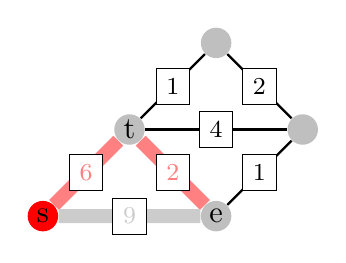
\begin{tikzpicture}[transform shape,label/.style={thin, draw=black, align=center,fill=white,font=\smaller},scale=1.1]
      \node[vertex] (a) at (0,0) {t};
      \node[vertex] (b) at (1,1) {};
      \node[vertex] (c) at (2,0) {};
      \node[vertex] (d) at (1,-1) {e};
      \node[red vertex] (e) at (-1,-1) {s};
      \draw[edge] (a) -- node[label] {$1$} (b);
      \draw[edge] (b) -- node[label] {$2$} (c);
      \draw[edge] (a) -- node[label] {$4$} (c);
      \draw[red edge] (a) -- node[label] {$2$} (d);
      \draw[edge] (c) -- node[label] {$1$} (d);
      \draw[red edge] (a) -- node[label] {$6$} (e);
      \draw[black edge] (d) -- node[label] {$9$} (e);
    \end{tikzpicture}
  \end{center}

  \bigskip

  In this graph, BFS would find $s \rightarrow e$ (cost 9) as the
  shortest path from $s$ to $e$, instead of $s \rightarrow t
  \rightarrow e$ (cost 8).
\end{frame}

\subsection{SSSP with Weighted Graph}
\begin{frame}
  \frametitle{Djikstra's Algorithm for weighted SSSP}
  \begin{block}{Basic Idea}
    Greedly selects the next edge that minimizes the total weight of the visited graph.
  \end{block}

  {\small
  \begin{itemize}
  \item Many different implementations (original paper has no implementation);
  \item A simple way is to use C++ stl's \emph{Priority Queue};
  \item When visiting a node, store new edges in the priority queue;
    {\smaller (priority queue sort edges as they are inserted)}
  \item For every new edge visited, check if new path on target node
    is cheaper than old one (if it is cheaper, visit the node again);
  \end{itemize}}
\end{frame}

\begin{frame}[fragile,singleslide]
  \frametitle{Djikstra's Algorithm: \_A\_ Implementation}
  {\smaller
    \begin{exampleblock}{}
\begin{verbatim}
Vector<int> dist(V,INF); dist[s] = 0;
priority_queue<ii, vector<ii>, greater<ii>> pq; 
pq.push(ii,(0,s));
while (!pq.empty()) {
   ii front = pq.top(); pq.pop(); 
   // shortest unvisited vertex
   int d = front.first; u = front.second;
   if (d > dist[u]) continue; // *lazy deletion*
   for (int j = 0; j < (int)AdjList[u].size(); j++) { 
      ii v = AdjList[u][j];
      if (dist[u] + v.second < dist[v.first]) { 
         dist[v.first] = dist[u] + v.second // relax
         pq.push(ii(dist[v.first],v.first));}}} 
         // new node to queue
\end{verbatim}
    \end{exampleblock}

    This implementation uses \emph{lazy deletion} to avoid deleting
    nodes from the queue unless absolutely necessary;}
\end{frame}

\begin{frame}
  \frametitle{Djikstra's implementation trick: Lazy deletion}
  {\smaller
    \begin{itemize}
    \item Djikstra Requires us to store the edge to vertex $v$ with
      cheapest weight in the queue;
    \item Removing an edge from the queue is expensive;
    \item Instead, we keep all edges, and test each visited edge;
    \end{itemize}
  

  % TODO: Redraw Djikstra graph by hand
  \begin{center}
    \includegraphics[width=0.6\textwidth]{../img/djikstra_halim}
  \end{center}

  Vertex queue: [\only<1>{(2,1),}\only<2>{(5,3),}
    \only<1-3>{(6,0),}\only<1-4>{(7,3),}
    \only<4->{(7,4),}\only<2->{(8,4),} \only<3->{(10,4)}];}

  \vfill 

  \hfill {\tiny Images from \emph{Competitive Programming}, Steven Halim}
\end{frame}

\subsection{Example: Full Tank?}
\begin{frame}
  \frametitle{Problem Example: UVA 11367 -- Full Tank} 
  {\smaller 
    A big part of Graph problems is figuring out the correct graph
    representation.

  \begin{block}{Problem Summary}
    In a graph $G$ of roads ($1 \leq V \leq 1000, 0 \leq E \leq
    10000$) with the following information:
    \begin{itemize}
    \item cost $l_{ij}$ in units of fuel between cities $i$ and $j$;
    \item price $p_{i}$ of buying fuel at city $i$;
    \item tank capacity $c$ of a car;
    \end{itemize}
    What is the least \structure{fuel price} from node $s$ to $e$; 
  \end{block}
  
   \begin{center}
    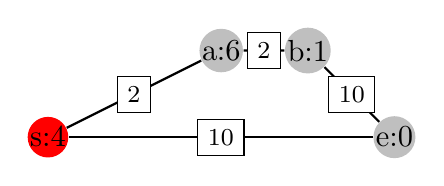
\begin{tikzpicture}[transform shape,label/.style={thin, draw=black, align=center,fill=white,font=\smaller},scale=1.1]
      \node[red vertex] (s) at (0,0) {s:4};
      \node[vertex] (0) at (2,1) {a:6};
      \node[vertex] (1) at (3,1) {b:1};
      \node[vertex] (e) at (4,0) {e:0};
      \draw[edge] (s) -- node[label] {$10$} (e);
      \draw[edge] (s) -- node[label] {$2$} (0);
      \draw[edge] (0) -- node[label] {$2$} (1);
      \draw[edge] (1) -- node[label] {$10$} (e);
    \end{tikzpicture}
  \end{center}
  
   The regular shortest path is $s$ to $e$, but the smallest fuel
   price is buying fuel at $s$ (cost 4) and at $a$ (cost 1), for a total cost 26}
\end{frame}

\begin{frame}
  \frametitle{UVA 11367 -- Full Tank -- Problem modeling}
  {\smaller
    \begin{center}
      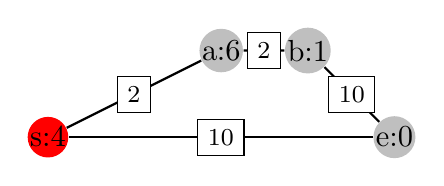
\begin{tikzpicture}[transform shape,label/.style={thin, draw=black, align=center,fill=white,font=\smaller},scale=1.1]
        \node[red vertex] (s) at (0,0) {s:4};
        \node[vertex] (0) at (2,1) {a:6};
        \node[vertex] (1) at (3,1) {b:1};
        \node[vertex] (e) at (4,0) {e:0};
        \draw[edge] (s) -- node[label] {$10$} (e);
        \draw[edge] (s) -- node[label] {$2$} (0);
        \draw[edge] (0) -- node[label] {$2$} (1);
      \draw[edge] (1) -- node[label] {$10$} (e);
      \end{tikzpicture}
    \end{center}
    
    \begin{block}{}
    Simple Djikstra on the $l_{ij}$ graph will not solve this problem,
    because we have to take into account the cost of buying fuel at
    different nodes.
    \end{block}
    
    \bigskip
    
    To model this problem, we modify the graph:
    \begin{itemize}
    \item Transform nodes $(i)$ into nodes $(i,f)$ (how much fuel left
      we have at $i$);
    \item An edge $(i,f)\rightarrow(j,f-l_{ij})$ exists if $f-l_{ij}
      \geq 0$ and has cost 0 (spend existing fuel);
    \item An edge $(i,f)\rightarrow(i,f+1)$ has cost $p_i$ (buy fuel at the city)
    \item Use regular djikstra on the new graph;
    \end{itemize}

  }
\end{frame}

\subsection{SSSP with Negative Cycle}
\begin{frame}
  \frametitle{Djikstra Problem with negative cycles}

  {\smaller
    \begin{block}{}
      The djikstra implementation suggested earlier \structure{can deal}
      with negative weights, but will enter an infinite loop if the graph
      has a \alert{negative loop}.
    \end{block}

    \begin{center}
      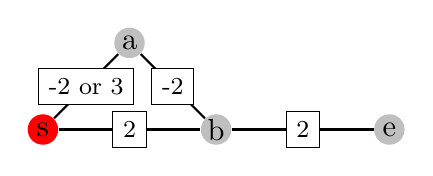
\begin{tikzpicture}[transform shape,label/.style={thin, draw=black, align=center,fill=white,font=\smaller},scale=1.1]
        \node[red vertex] (s) at (0,0) {s};
        \node[vertex] (0) at (1,1) {a};
        \node[vertex] (1) at (2,0) {b};
        \node[vertex] (e) at (4,0) {e};
        \draw[edge] (s) -- node[label] {-2 or 3} (0);
        \draw[edge] (s) -- node[label] {2} (1);
        \draw[edge] (1) -- node[label] {-2} (0);
      \draw[edge] (1) -- node[label] {2} (e);
      \end{tikzpicture}
    \end{center}
    
    \begin{itemize}
    \item The Djikstra implementation above will keep adding negative
      nodes as smaller totals are generated: -2, -4, -6, -8...
    \item The Problem is that it does not include an explicit check
      for \emph{non-simple} paths;
    \item To deal with negative loops, one alternative is the
      \structure{Bellman Ford's algorithm}
    \end{itemize}
  }
\end{frame}

\begin{frame}[fragile,singleslide]
  \frametitle{Bellman Ford's Algorithm $O(VE)$}

  {\smaller
  \structure{Main Idea}: Relax all $E$ edges in the graph $V-1$ times;

  \begin{exampleblock}{}
\begin{verbatim}
vector<int> dist(V, INF); dist[s] = 0;
for (int i = 0; i < V - 1; i++) // repeat V-1 times
 for (int u = 0; u < V; u++) // for all vertices
  for (int j = 0; j < (int)AdjList[u].size(); j++) {
    ii v = AdjList[u][j]; // record path here if needed;
    dist[v.first] = min(dist[v.first], dist[u]+v.second);
    } //relax edge
\end{verbatim}
  \end{exampleblock}
  
  \medskip

  \structure{How does it work?}:
  \begin{itemize}
  \item At the start, \emph{dist[s]} has the correct minimal distance;
  \item When relax all edges, at least one node now has correct minimal distance;
  \item After \emph{V-1} iterations, all nodes have correct minimal distances;
  \end{itemize}
  }
\end{frame}

\begin{frame}
  \frametitle{A bit more on Bellman Ford's}
  {\smaller
  \begin{block}{Detecting Negative Loops}
    Bellman Ford's algorithm can be used to detect if a negative loop
    exists in the graph.  

    \medskip

    \begin{itemize}
      \item Execute the algorithm once. 
      \item Do one last round of ``relax all nodes''. 
      \item If any distance in the \emph{dist[]} vector changes, the graph has a negative loop.
    \end{itemize}
  \end{block}}
\end{frame}


\begin{frame}
  \frametitle{Summary of SSSP}
  \begin{itemize}
  \item \structure{BFS}: $O(V+E)$, only for unweighted graphs
  \item \structure{Djikstra}: $O(E+V\text{log}V)$, problem with negative loops
  \item \structure{Bellman Ford}: $O(EV)$, can find negative loops\\(simple to code)
  \end{itemize}

  \bigskip

  Study/Implement all of them, but always use the simplest possible!
\end{frame}


\section{APSP}
\subsection{All Pairs Shortest Path}
\begin{frame}
  \frametitle{APSP: All Pairs Shortest Path}

  {\smaller
  \begin{block}{Problem Definition -- UVA 11463 -- Commandos}
    Given a graph $G(V,E)$, and two vertices $s$ and
    $e$, calculate the smallest possible value of the path $s
    \rightarrow i \rightarrow e$ for every node $i \in V$.
  \end{block}

  \begin{itemize}
  \item One way to do it would be for every node $i$, calculate
    Djikstra(s,i) + Djikstra(i,e);
  \item This would cost $O(V(E+V\text{log}(V)))$;
  \item If the graph is \structure{small} $(|V| \leq 400)$, there is a
    simpler-to-code algorithm that costs $O(V^3)$
  \end{itemize}
  }
\end{frame}

\begin{frame}[fragile,singleslide]
  \frametitle{The Floyd-Warshall Algorithm -- $O(V^3)$}

{\smaller

  \begin{exampleblock}{}
\begin{verbatim}
int AdjMat[V][V]; 
//contains weight of edge(i,j) or INF if no such edge

for (int k=0; k < V; k++) // loop order is k -> i -> j
   for (int i=0; i < V; i++)
      for (int j=0; j < V; j++)
         AdjMat[i][j] = min(AdjMat[i][j],
                            AdjMat[i][k]+AdjMat[k][j]);
// AdjMat[i][j] now contains the minimal cost[i][j]
\end{verbatim}
  \end{exampleblock}

  \begin{itemize}
  \item Computational cost is more expensive than $V$ times
    Djikstra;
  \item \alert{Programmer Cost} is clearly cheaper than Djikstra
    or Bellman-Ford;
  \end{itemize}
}
\end{frame}

\begin{frame}
  \frametitle{Why does Floyd Warshall work?}

  {\smaller
  \begin{block}{Basic Idea: Bottom-up Dynamic Programming}
    FW uses this recursive idea: ``The shortest path S between $i$ and
    $j$ is either $S(i,j)$, or $S(i,v) + S(v,j)$ for all nodes $v$
    between $0$ to $k$.''

    \medskip

    \begin{itemize}
    \item $k=-1$ is the base case, $S$ is the edge ($i,j$);
    \item For $k=n$, the shortest path uses $S(i,v,n-1)$ and
      $S(v,j,n-1)$;
    \end{itemize}
  \end{block}
  }
  
  \begin{center}
    \includegraphics<1>[width=0.7\textwidth]{../img/fw_halim1}
    \includegraphics<2>[width=0.7\textwidth]{../img/fw_halim2}
    \includegraphics<3>[width=0.7\textwidth]{../img/fw_halim3}
    \includegraphics<4>[width=0.7\textwidth]{../img/fw_halim4}
  \end{center}

  \medskip

  \hfill {\tiny Images from \emph{Competitive Programming}, Steven Halim}
\end{frame}

\subsection{Tricks with ASPS}
\begin{frame}
  \frametitle{Tricks with ASPS}

  % TODO: Write down each trick with details, write code;
  \begin{itemize}
  \item Include parents: Add a 2D parent matrix, which is updated in
    the inner loop; Follow the parent matrix backwards when the
    execution is over;
  \item Connectivity: If all we want to know if is $i$ is connected to
    $j$, do FW with bitwise operations (FW[i][j] = FW[i][k] \&\&
    FW[k][j]) -- much faster!
  \item Finding SCC: If FW[i][j] and FW[j][i] are both $> 0$, then $i$
    and $j$ belong to the same SCC;
  \item Minimum Cycle/Negative Cycle: Check the diagonal of FW:
    $FW[i][i] < 0$;
  \item ``Diameter'' of a Graph: $i,j$ where $FW[i][j]$ is maximum;
  \end{itemize}
\end{frame}

\subsection{Problem Discussion}
\begin{frame}
  \frametitle{SSSP and ASPS problem discussion}
  % TODO: Add discussion of problems
  {\smaller
  \begin{itemize}
    \item From Dusk Until Down;
    \item Wormholes; 
    \item Mice and Maze; 
    \item Degrees of Separation;
    \item Avoiding your Boss;
    \item Arbitrage;
  \end{itemize}}
\end{frame}

\section{Network Flow}
\subsection{Network Flow}
\begin{frame}
  \frametitle{Network Flow}

% Motivation: Imagine a connected, weighted and directed graph as a network of pipes. 
% From the source node, an infinite amount of water is entering. How much water is leaving
% At the destination node?

%% TODO: Water Flow image

% This problem is called the MAX FLOW problem, in a family of problems
% involving flow in networks
\end{frame}

\begin{frame}[fragile,singleslide]
  \frametitle{Ford Fulkerson Method}
  One way to solve the Max Flow is the Ford Fulkerson Method (Footnote: Same Ford as the Bellman-Ford algorithm)

Algorithm Idea:
\begin{verbatim}
// initial setup: residual graph - edge capacity = original edge weight
mf =0
while ("a path p with positive weight exists" from s to t):
  find v (edge with minimal weight in p)
  remove Wv from all foward edges i in P(s,g)
  increase Wv to all backward edges i in P(g,s)
  mf += f
} 
\end{verbatim}

Question to think about: Why do we increase Wv to all backward edges?
\end{frame}

\begin{frame}
  \frametitle{Implementing Ford Fulkerson Method}
``while (a path p with positive weight exists)``

How do we find this path? Examples: BFS, DFS.
(Does not need to be minimal, the increase of Wv will fix that (but it may be slow))

Cost with DFS: O(|f*|E), where f* is the Max Flow value. But f* can be arbitrarily large!

Better idea: BFS (Edmond Karp's algorithm)
\end{frame}

\begin{frame}[fragile,singleslide]
  \frametitle{Edmond Karp's algorithm implementation}

%% Page 190, O(V^3E), can be made better by optimizing the code (more complicated)
\end{frame}

\begin{frame}
  \frametitle{Network Flow Problem Example: UVA 259}
\end{frame}

\begin{frame}
  \frametitle{Network Flow Problem Variants}
  %% Minimum Cut: Find a minimum set of edges C so that if all sets are removed the flow 
  % from sourse s to sink e becomes 0 (i.e., s and t are disconnected)

  % all nodes reachable from source on edges with positive residual are connected to St,
  % all nodes not reachable from source on edges with positive residual are connected to En,
  % all edges with residual = 0, connecting the two sets S,E, belong to the min cut

  %% Multi-source, multi-sink: create a super source node ss, and a super sink node ee, which
  % connect to all sources/all sinks one-way with infinite weights.

  %% Weights on vertex: we can modify the graph by splitting the vertices, and connecting 
  % i1 to i2 with the vertex weight. Beware, because this increases V ans E
\end{frame}

% TODO: Graph modeling example, page 193, titanic sample problem
% TODO: Converting Graph to DAG, solving SSSP on DAG: Fishmonger - node cost + goal time
% (Not really network flow -- bonus problems on graphs/revisiting DP)


\section{Special Graphs}
\subsection{Special Graphs}
% TODO: Replaced ``bipartite Match'' with special graphs, deal with many examples from 4.7.*

\begin{frame}
  \frametitle{Graph Problems: Thinking with many boxes} 

  The interesting part about graph problems is that they came in great
  variety. Once you know the basic algorithms, the main problem is figuring
  out what kind of graph you are dealing with.

  This knowlege only comes with practice, but here are some examples.
\end{frame}

\begin{frame}
  \frametitle{DAG example: Timed SSSP}
  % TODO: Converting Graph to DAG, solving SSSP on DAG: Fishmonger - node cost + goal time
\end{frame}

\begin{frame}
  \frametitle{Max Flow Example: Iceberg}
  % TODO: Graph modeling example, page 193, titanic sample problem
\end{frame}

\begin{frame}
  \frametitle{Bipartite Example - Prime pairing}
  % Page 208
\end{frame}

\begin{frame}
  \frametitle{Flow and Special Graph problems}
\end{frame}

\section{Conclusion}
\subsection{Conclusion}
\begin{frame}
  \frametitle{Summary}
\end{frame}

\begin{frame}
  \frametitle{This Week's Problems}
\end{frame}

\begin{frame}
  \frametitle{Next Weeks}
  \begin{itemize}
  \item Week 7
  \item Week 8
  \item Week 9
  \end{itemize}
\end{frame}

\end{document}

